\def\SCALE{.85}
\begin{tikzpicture}[,scale=\SCALE,font=\sffamily\fontsize{8}{8}\selectfont]
  \def\WDTA{3in}
  \def\WDTB{2in}
  \def\WDTC{2.35in}
  \def\WDTD{3in}
  \def\DCOL{black!8}
  \def\DCOLS{black}
  \def\ECOLA{black!5}
  \def\ECOLB{black!5}
  \def\ECOLC{Green4!5}
  \def\ECOLD{Green4!5}
  \def\LWD{2pt}
  \def\LWDA{6pt}
  \def\ACOL{black}
  \def\OPC{.7}
  \def\OPCA{.95}
  \def\OPCB{.15}
  \def\CIRC{circle}
 % \clip (3.25in,0.02in) rectangle (-4.1in,-8.95in);
  \node[] (N0) at (0,0) {};
 
\node[anchor=north east] (N1) at ([xshift=.75in,yshift=0in]N0.north west) {
%
  \begin{tikzpicture}[anchor=east,scale=\SCALE,]
\tikzset{xcirc/.style={circle,fill=\ECOLB,opacity=\OPC,rounded corners=5pt,draw=\DCOL,line width=\LWD,scale=\SCALE}}
\tikzset{xcircs/.style={circle,fill=none,opacity=1,rounded corners=5pt,draw=none,ultra thick,,scale=\SCALE}}
\tikzset{xdr/.style={\ACOL,line width=\LWDA, opacity=\OPCA}}
    \node[xcirc,inner sep=-20pt,label={[yshift=.5in,distance=0in,align=center]-90:Predictor for\\index 1274}] (P1274) at (0,0) {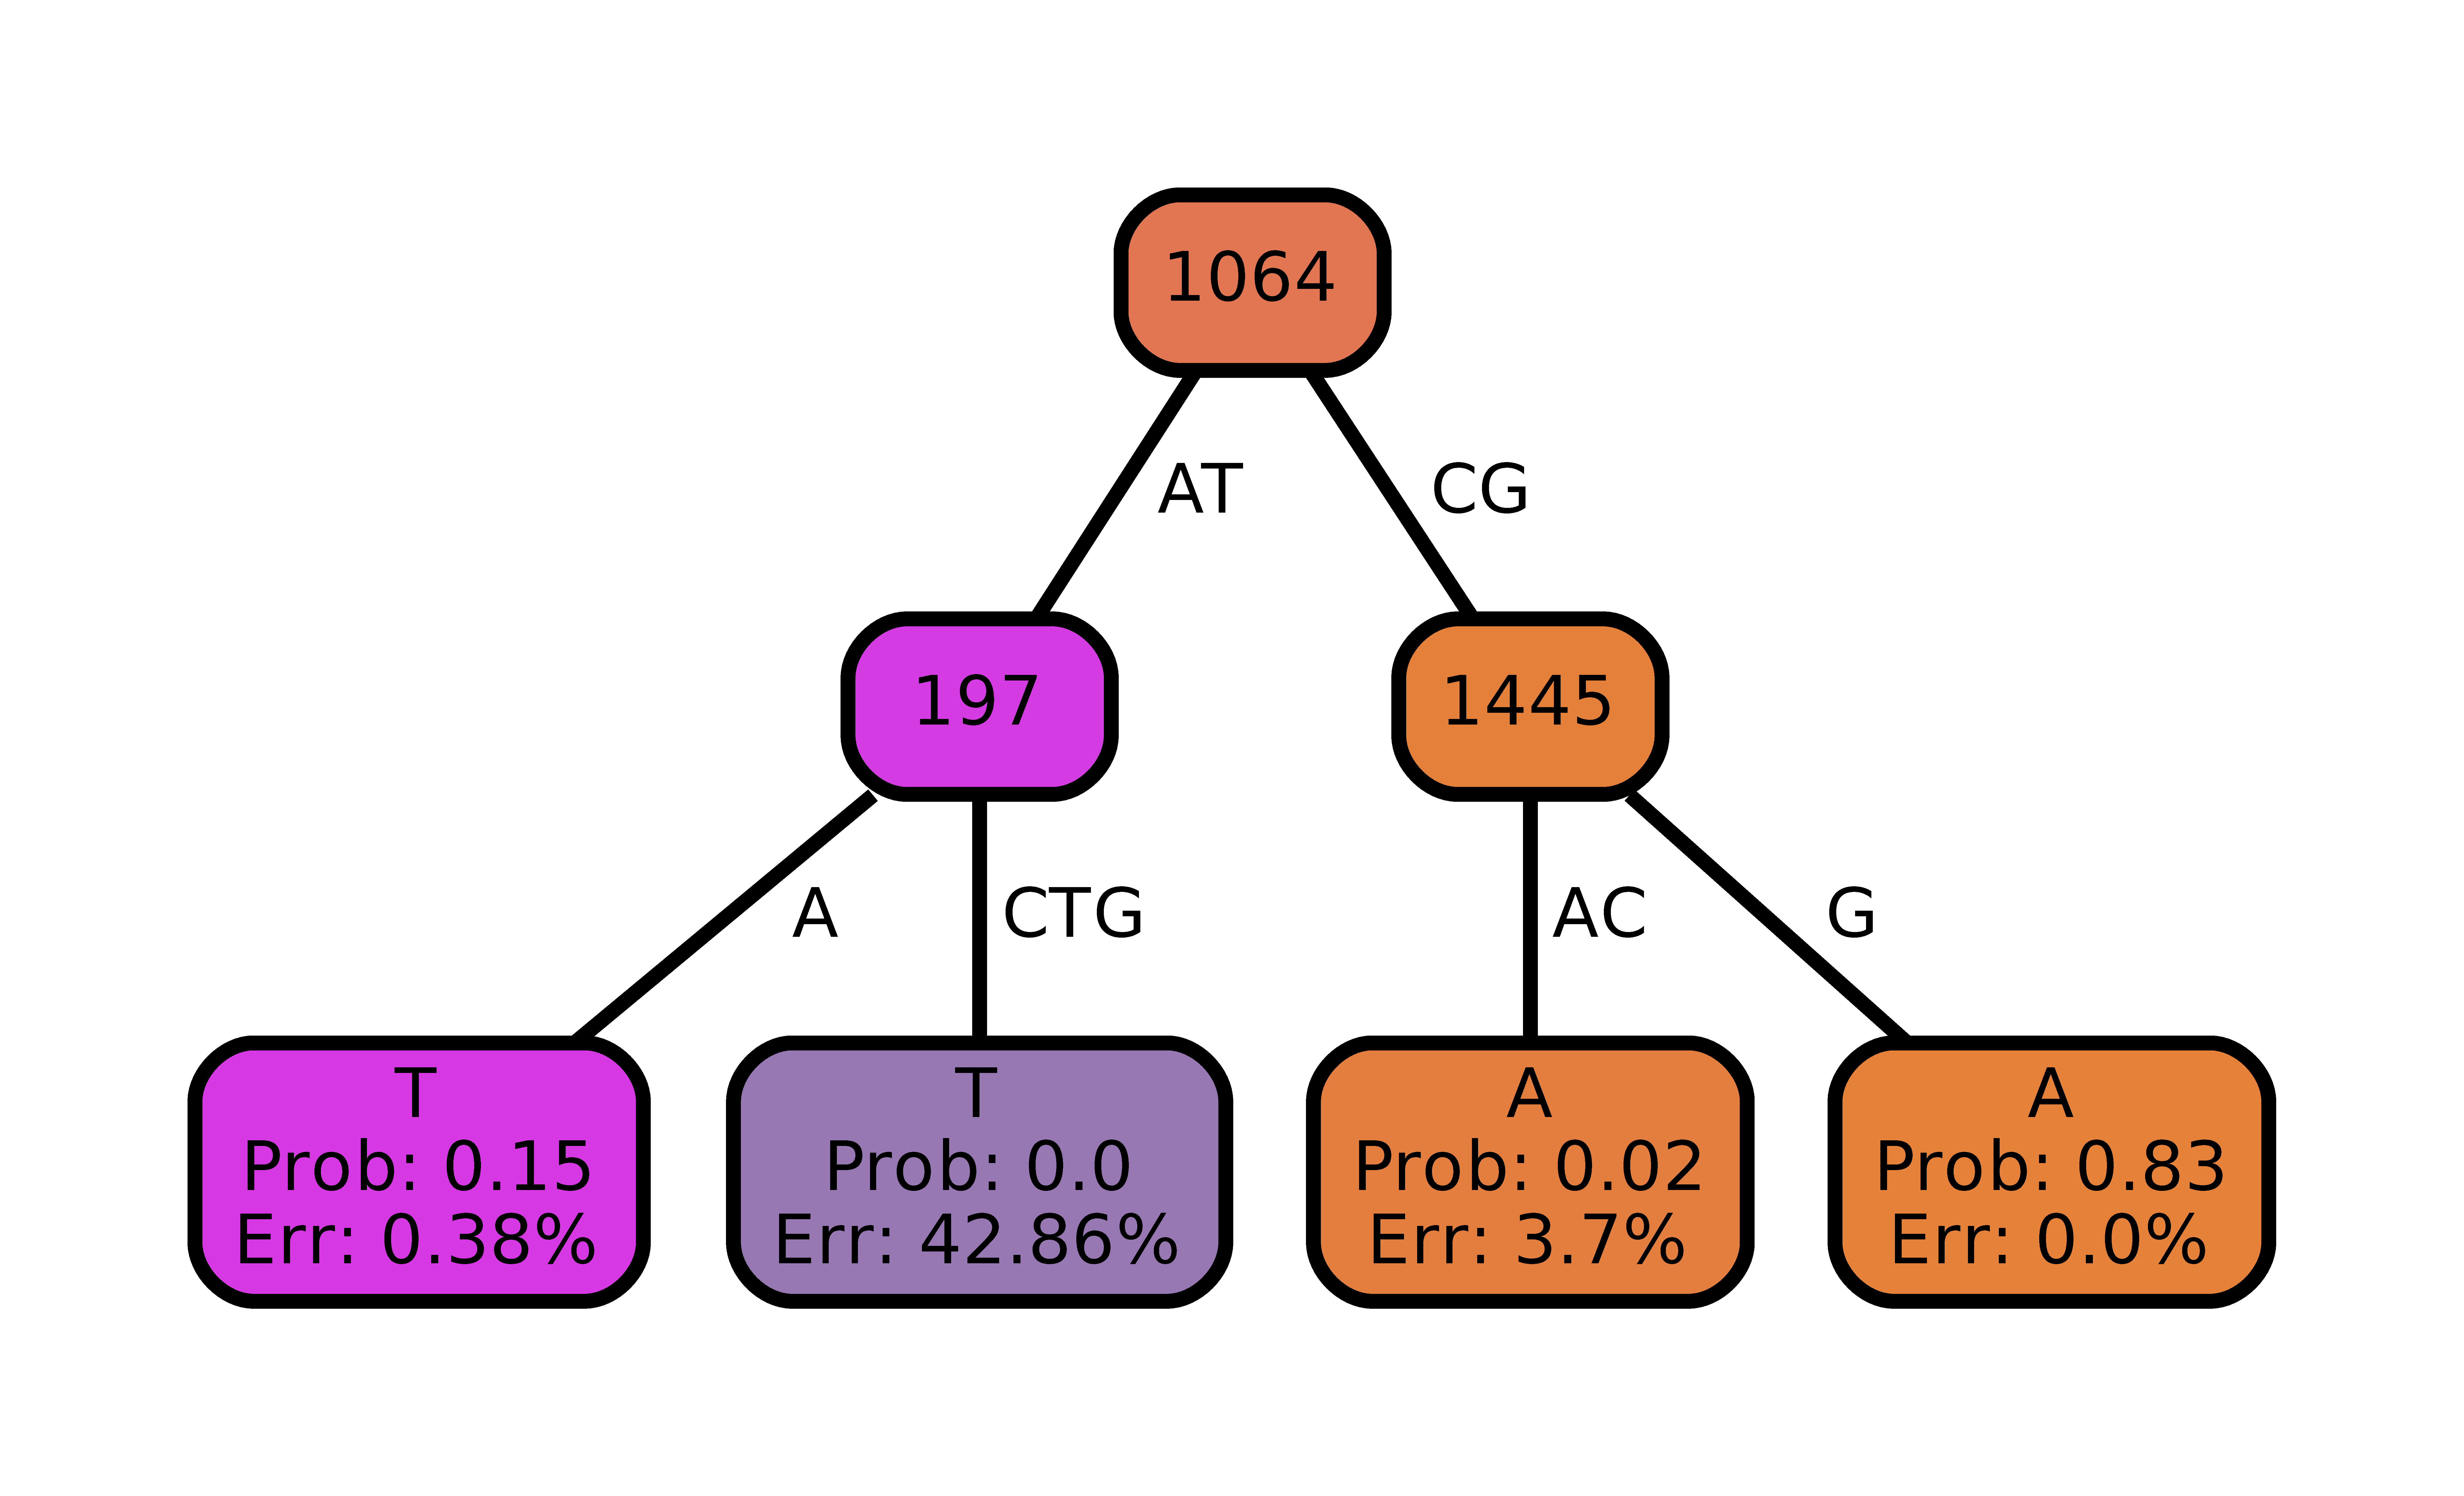
\includegraphics[width=\WDTA]{Figures/plotdata/TREE_P1274}};
    \node[xcirc,inner sep=-12pt,anchor=south,label={[yshift=.35in,distance=-.75in,align=center]-90:Predictor for\\index 1064}] (P1064) at ([xshift=.5in,yshift=-.65in]P1274.north) {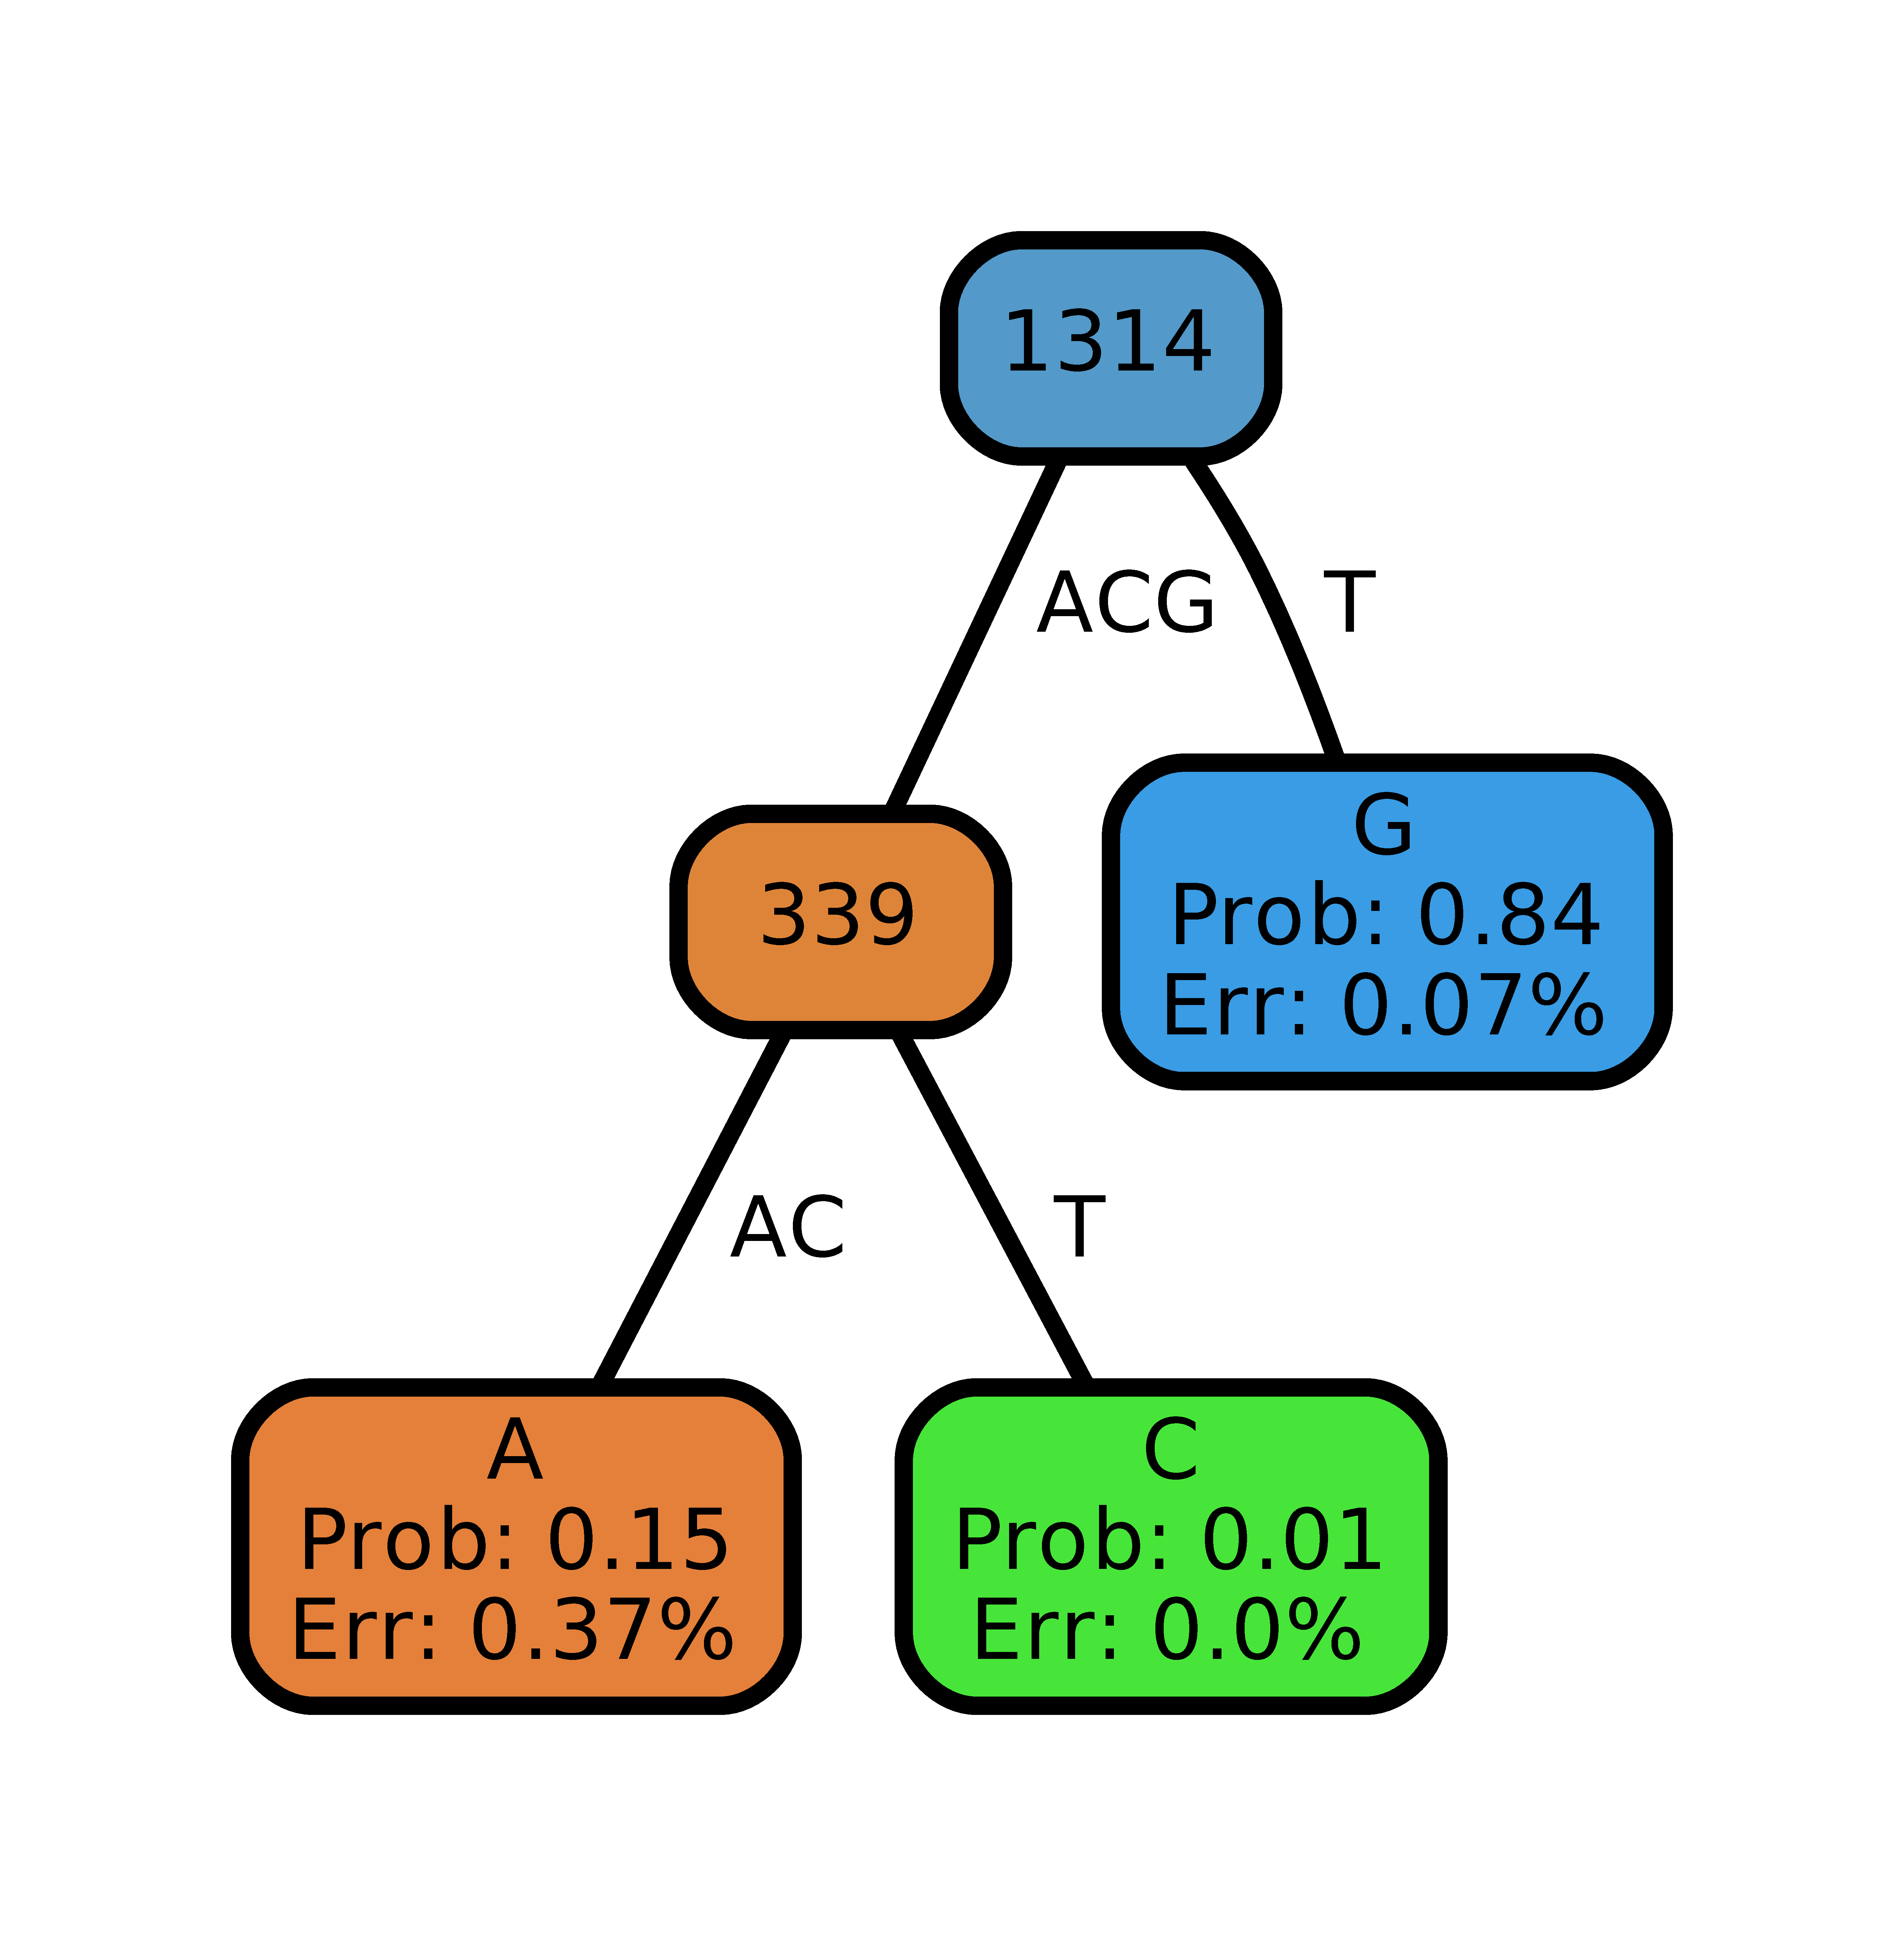
\includegraphics[width=\WDTB]{Figures/plotdata/TREE_P1064}};
     \node[xcirc,inner sep=-17pt,anchor=east,label={[xshift=.75in,yshift=.25in,distance=-.75in,align=center]-145:Predictor for\\index 1314}] (P1314) at ([xshift=2.25in,yshift=2.2in]P1064.west) {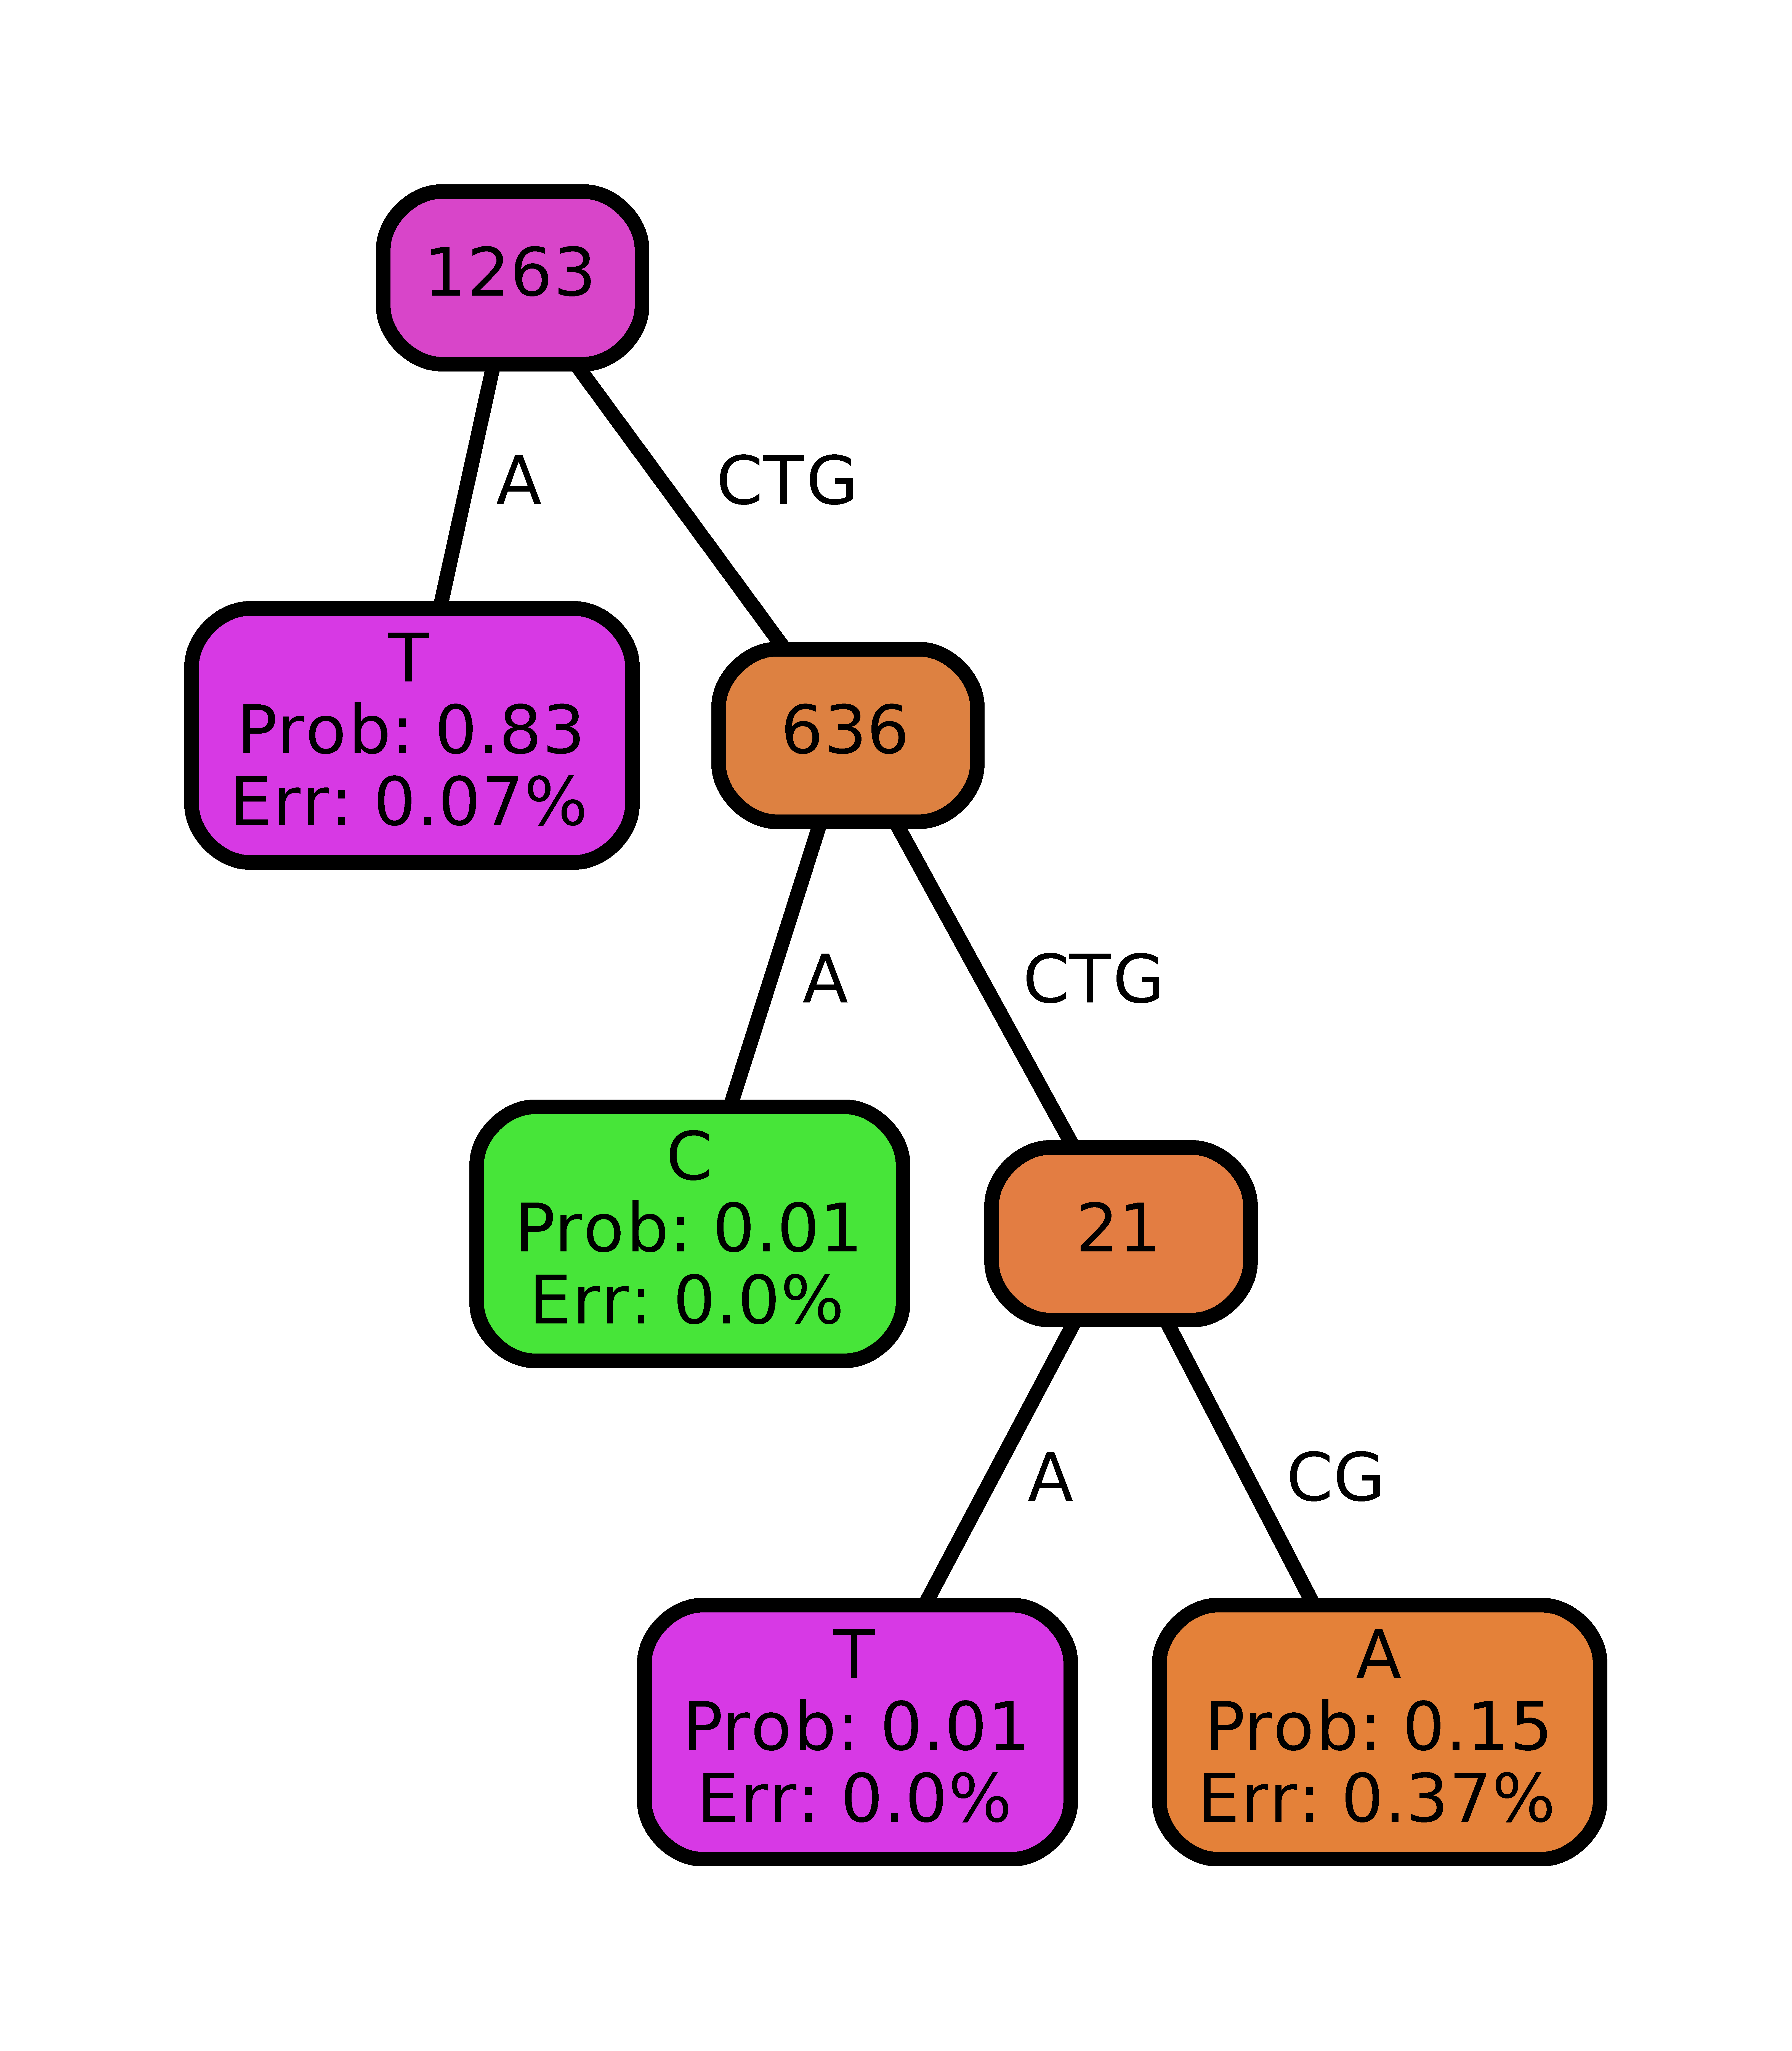
\includegraphics[width=\WDTC]{Figures/plotdata/TREE_P1314}};
    % \node[xcirc,inner sep=-12pt,anchor=south west,label={[yshift=.5in,distance=-.75in,align=center]-90:Predictor for\\index 1263}] (P1263) at ([xshift=-.35in,yshift=-.4in]P1314.north east) {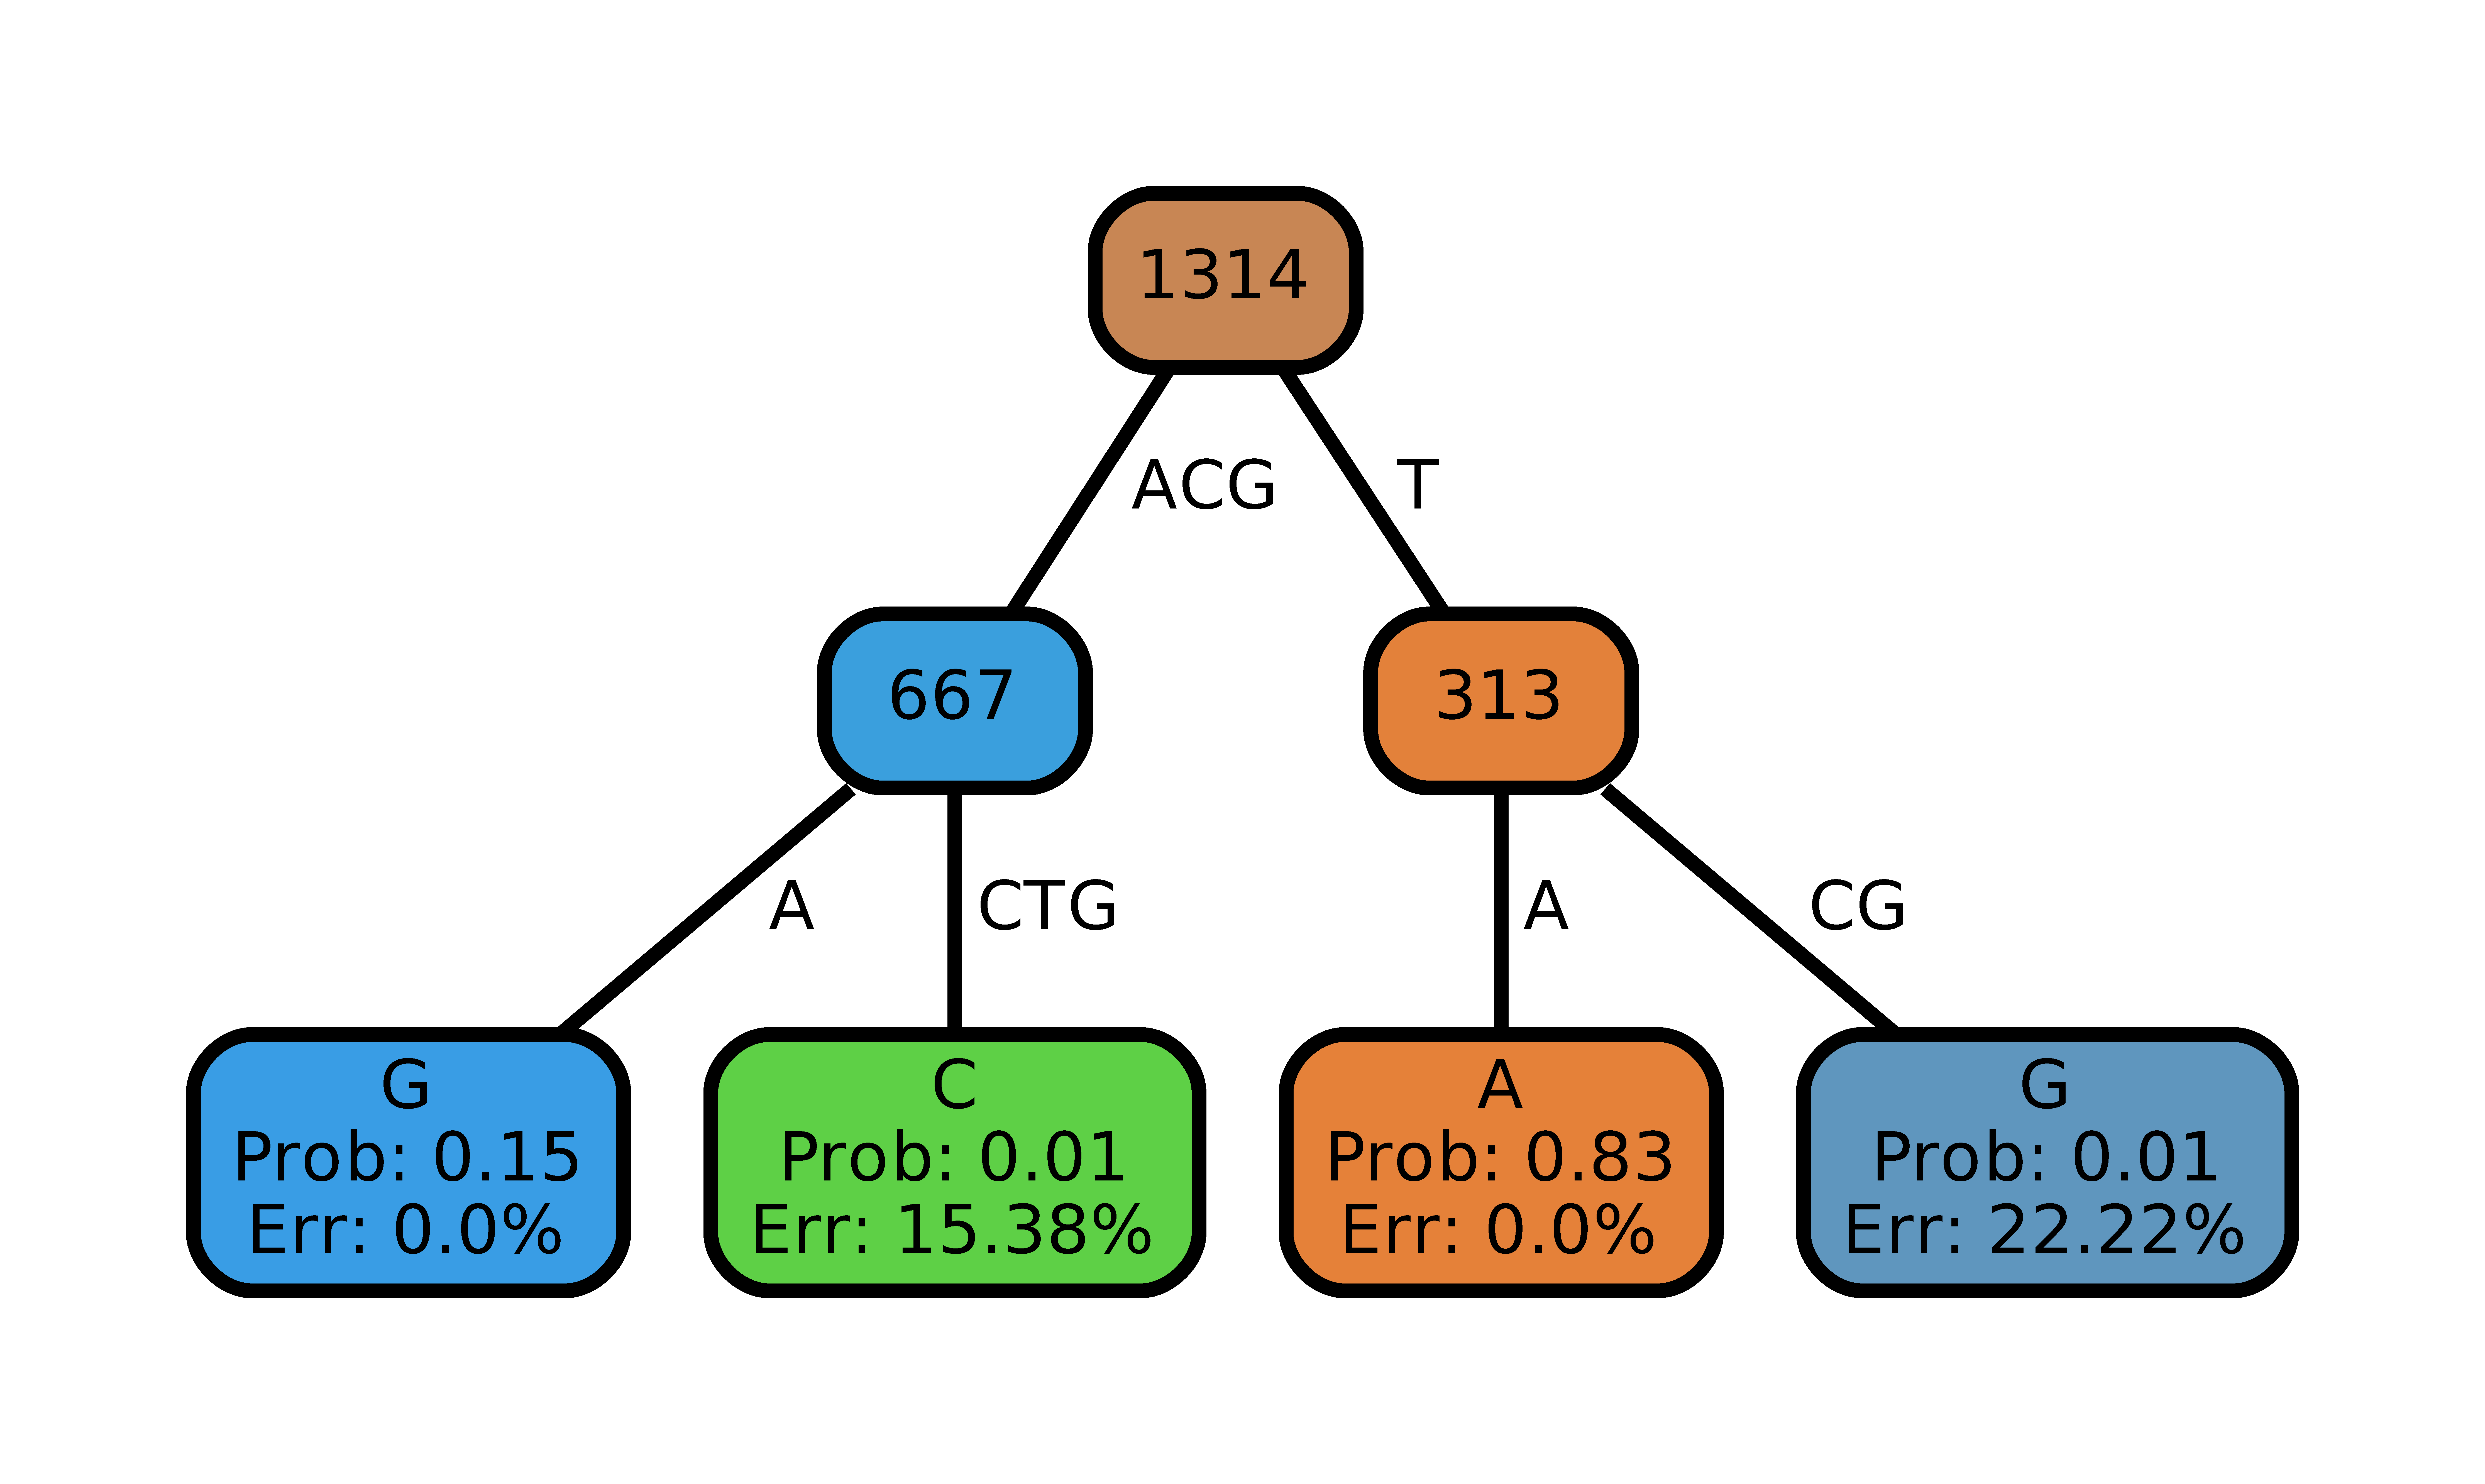
\includegraphics[width=\WDTD]{Figures/plotdata/TREE_P1263}};

\node[xcircs,inner sep=10.5pt] (N1) at ([yshift=.575in,xshift=.25in]P1274) {};
\node[xcircs,inner sep=11pt] (N2) at ([yshift=.985in,xshift=-0.27in]P1314) {};
\node[xcircs,inner sep=11pt] (N3) at ([yshift=.67in,xshift=0.4in]P1064) {};
%\node[xcircs,inner sep=10.5pt] (N4) at ([yshift=.57in,xshift=0.2in]P1263) {};
    %\draw [xdr,-{Latex[length=10mm]}] (N1) -- (P1064);
    %%\draw [xdr,,-{Latex[length=10mm]}] (N2) -- (P1263);
    %\draw [xdr,,-{Latex[length=10mm]}] (N3) -- ([xshift=.8in]P1314.center);
    %\draw [xdr,,-{Latex[length=10mm]}] (N4) to [out=145,in=90,looseness=1.45] (P1314);

\node[font=\bf\sffamily,anchor=east,rounded corners=3pt,align=center] (I1) at ([yshift=2.75in,xshift=.75in]P1274.west) {Color\\key$^\bigstar$};

\node[font=\bf\sffamily,anchor=north,rounded corners=3pt,text width=.1in,text height=.1in,fill=Purple1,align=center] (I1) at (I1.south) {T};

\node[font=\bf\sffamily,anchor=north,rounded corners=3pt,text width=.1in,text height=.1in,fill=DarkOrange3!70,align=center] (I1) at (I1.south) {A};

\node[font=\bf\sffamily,anchor=north,rounded corners=3pt,text width=.1in,text height=.1in,fill=SeaGreen2,align=center] (I1) at (I1.south) {C};

\node[font=\bf\sffamily,anchor=north,rounded corners=3pt,text width=.1in,text height=.1in,fill=DodgerBlue2!80,align=center] (I1) at (I1.south) {G};

%\node[font=\bf\sffamily\fontsize{4}{5},anchor=north west,align=left,text=gray] (I1) at ([yshift=-.1in,xshift=-.1in]I1.south west) {
%{\large$^\bigstar$}Mixed colors represent\\distribution over different\\nucleotide outcomes
%};
    \end{tikzpicture}
  };
% \def\WDT{2.25in}
%  \node[anchor=south west] (Nf1) at ([xshift=-.15in,yshift=-.35in]N1.south east) {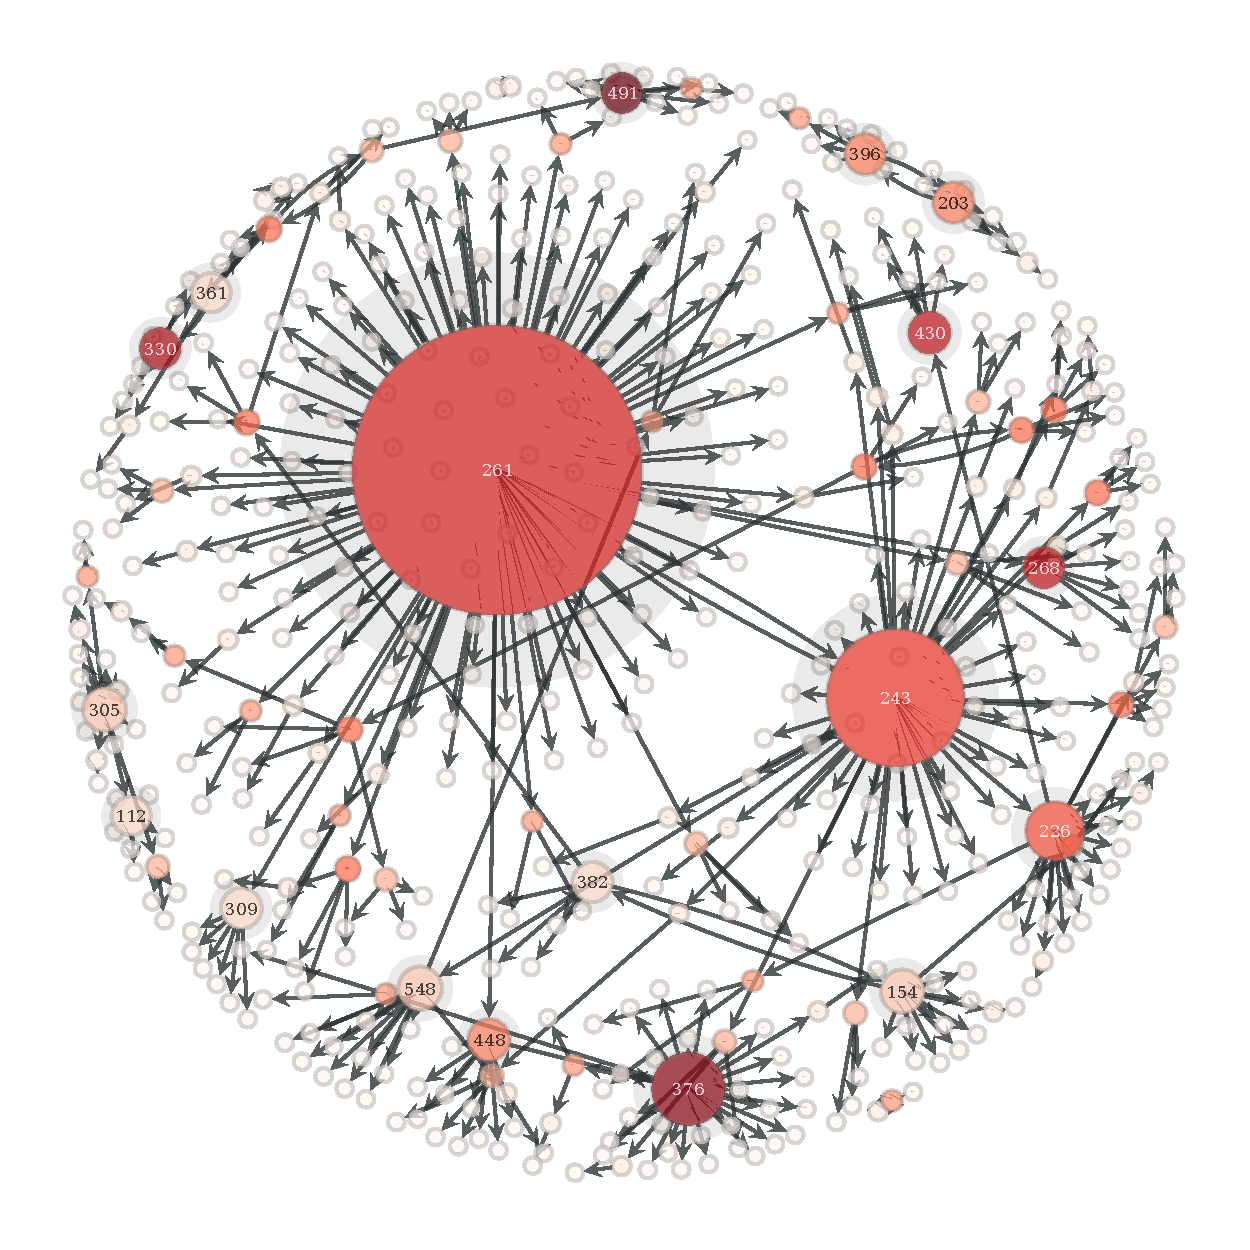
\includegraphics[width=\WDT]{Figures/qfig/output_human2009_2010}};

  % \def\LWD{5pt}
  % \node[anchor=north,align=left,font=\bf\tt\footnotesize] (N3) at ([yshift=-.1in,xshift=-0in]N1.south) {\bf\sffamily\fontsize{7}{8}\selectfont Influenza A 2018\\\bf\sffamily\fontsize{7}{8}\selectfont Haemagglutinin Sequences\\GGAAAACAAAAGCAACAAAA$\cdots$TGA{\large\color{Red1} A}AAAAGA$\cdots$\\AGCAAAAGCAGGGGAAAACA$\cdots $GTT{\large\color{Red1}C}AACCAC$\cdots$\\AGCAAAAGCAGGGGAAAACA$\cdots$GTT{\large\color{Red1}T}AACCAC$\cdots$\\ATGAAGACTATCATTGCTTT$\cdots$ACC{\large\color{Red1}T}TGAGAA$\cdots$};

% \node[anchor=west,align=left,font=\bf\sffamily\fontsize{8}{10}\selectfont] (N4) at ([xshift=.2in]N3.east) {A/Italy/7366/2018\\
% A/Baltimore/P0264/2018\\
% A/Baltimore/P0278/2018\\  
% A/Florida/61/2018};

% \draw [ultra thick] ([yshift=.25in,xshift=.01in]N4.west) --++ (-.23in,-.19in);
% \draw [ultra thick] ([yshift=.1in,xshift=.01in]N4.west) --++ (-.23in,-.2in);
%  \draw [ultra thick] ([yshift=-0.05in,xshift=.01in]N4.west) --++ (-.23in,-.2in);
%  \draw [ultra thick] ([yshift=-.2in,xshift=.01in]N4.west) --++ (-.23in,-.2in);

%\draw [-{Latex[length=10mm]},ultra thick,line width=\LWD,\ACOL] ([xshift=-.1in,yshift=-.25in]N3.north) --++(0,.8in) node [yshift=-1.25in,below,align=center,text=IndianRed2] {residue\\1274};


 \node[anchor=north west] (A1) at ([xshift=-3in,yshift=1.6in]N1.north east) {
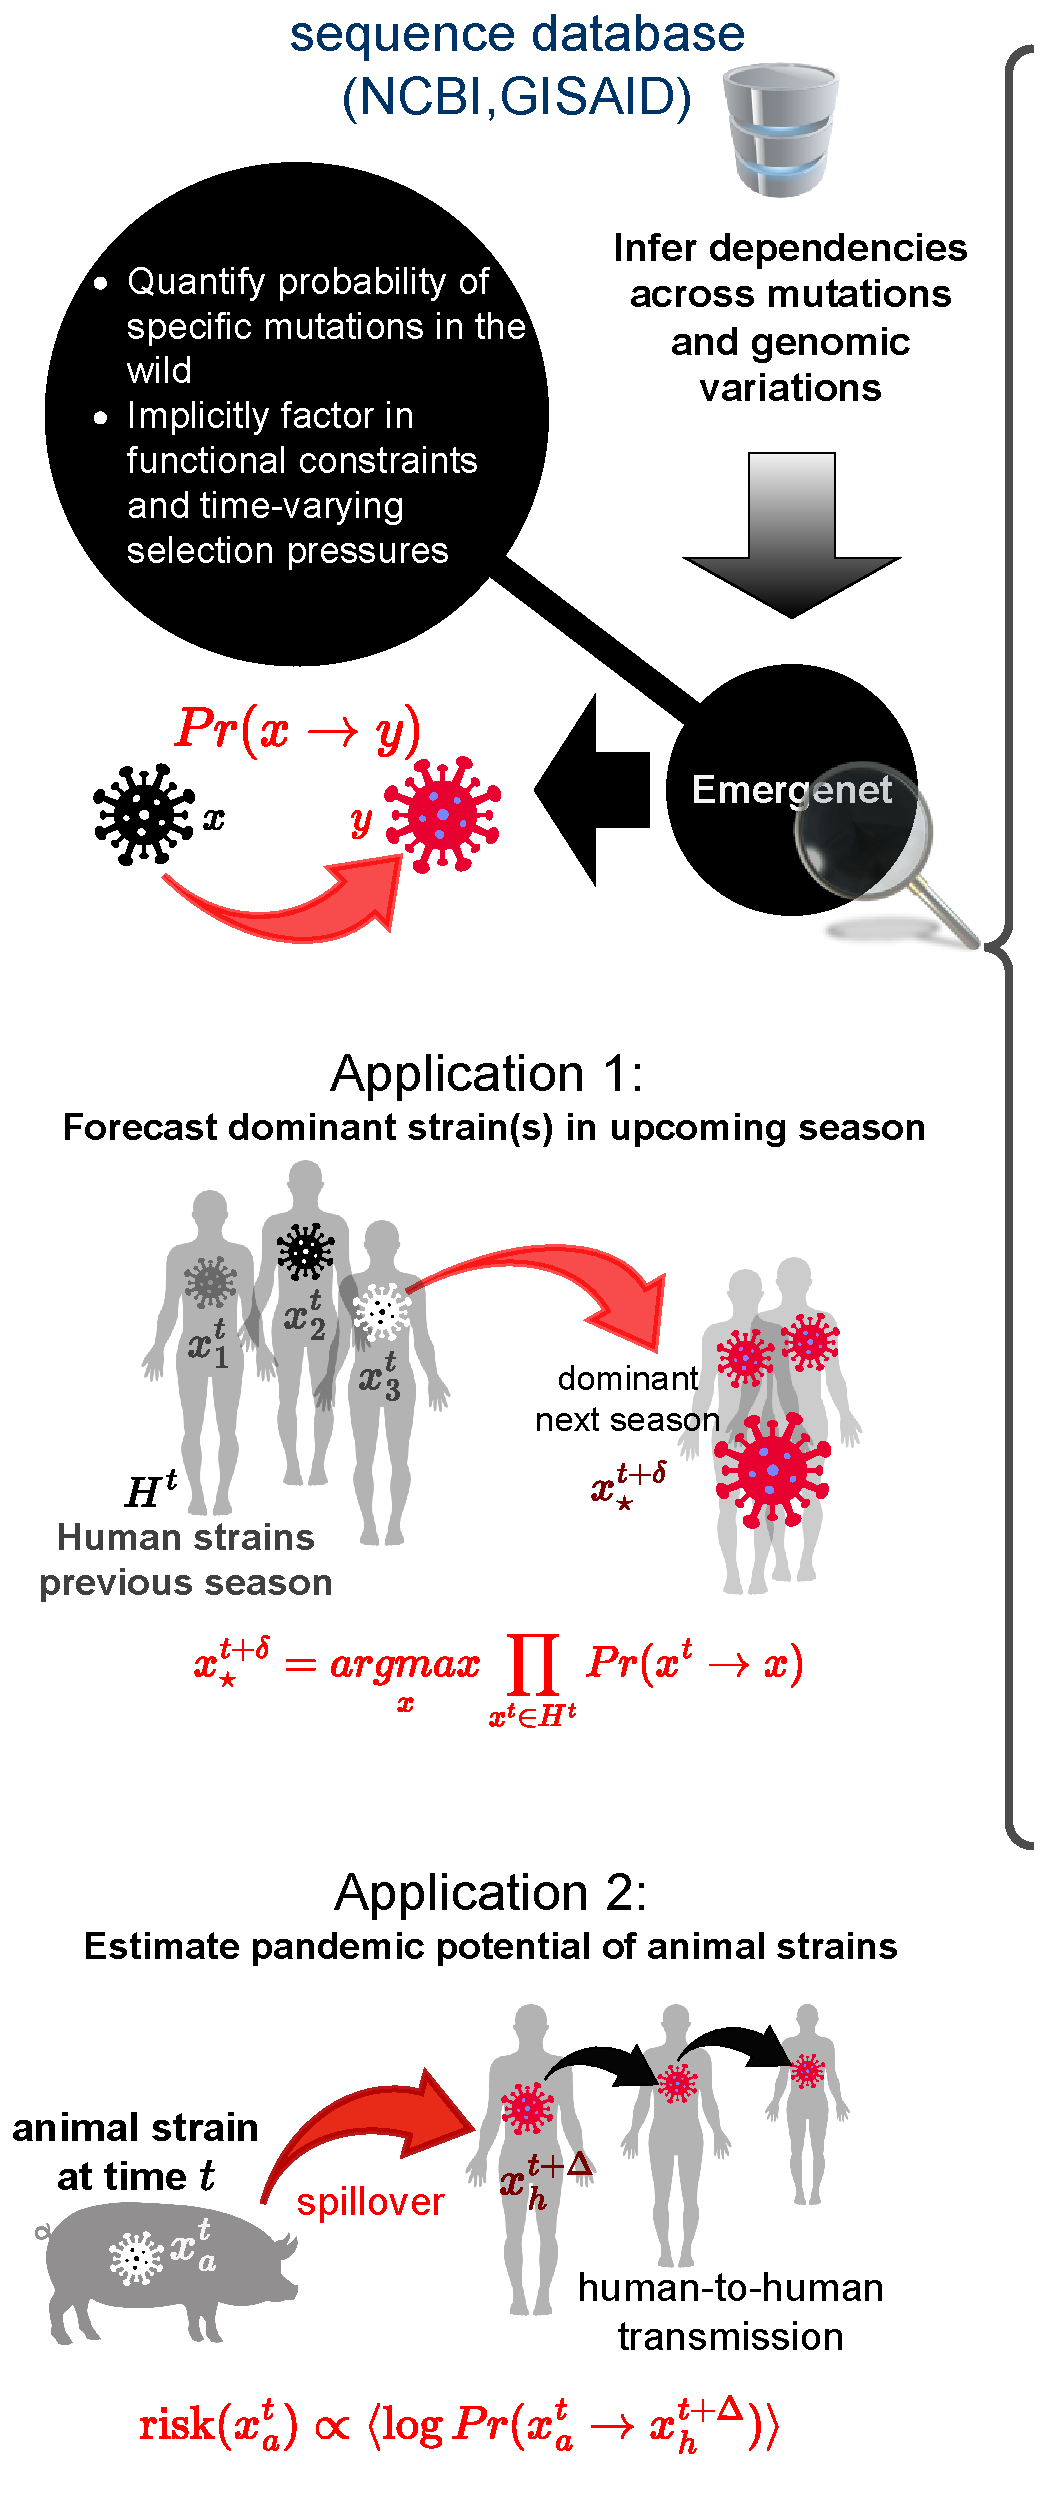
\includegraphics[width=6.0in]{Figures/e2}
 };
  
\end{tikzpicture}
